\documentclass[12pt]{article}

% \usepackage{amsmath}
%\widebar command from https://tex.stackexchange.com/a/60253/286191
\makeatletter
\let\save@mathaccent\mathaccent
\newcommand*\if@single[3]{%
  \setbox0\hbox{${\mathaccent"0362{#1}}^H$}%
  \setbox2\hbox{${\mathaccent"0362{\kern0pt#1}}^H$}%
  \ifdim\ht0=\ht2 #3\else #2\fi
  }
%The bar will be moved to the right by a half of \macc@kerna, which is computed by amsmath:
\newcommand*\rel@kern[1]{\kern#1\dimexpr\macc@kerna}
%If there's a superscript following the bar, then no negative kern may follow the bar;
%an additional {} makes sure that the superscript is high enough in this case:
\newcommand*\widebar[1]{\@ifnextchar^{{\wide@bar{#1}{0}}}{\wide@bar{#1}{1}}}
%Use a separate algorithm for single symbols:
\newcommand*\wide@bar[2]{\if@single{#1}{\wide@bar@{#1}{#2}{1}}{\wide@bar@{#1}{#2}{2}}}
\newcommand*\wide@bar@[3]{%
  \begingroup
  \def\mathaccent##1##2{%
%Enable nesting of accents:
    \let\mathaccent\save@mathaccent
%If there's more than a single symbol, use the first character instead (see below):
    \if#32 \let\macc@nucleus\first@char \fi
%Determine the italic correction:
    \setbox\z@\hbox{$\macc@style{\macc@nucleus}_{}$}%
    \setbox\tw@\hbox{$\macc@style{\macc@nucleus}{}_{}$}%
    \dimen@\wd\tw@
    \advance\dimen@-\wd\z@
%Now \dimen@ is the italic correction of the symbol.
    \divide\dimen@ 3
    \@tempdima\wd\tw@
    \advance\@tempdima-\scriptspace
%Now \@tempdima is the width of the symbol.
    \divide\@tempdima 10
    \advance\dimen@-\@tempdima
%Now \dimen@ = (italic correction / 3) - (Breite / 10)
    \ifdim\dimen@>\z@ \dimen@0pt\fi
%The bar will be shortened in the case \dimen@<0 !
    \rel@kern{0.6}\kern-\dimen@
    \if#31
      \overline{\rel@kern{-0.6}\kern\dimen@\macc@nucleus\rel@kern{0.4}\kern\dimen@}%
      \advance\dimen@0.4\dimexpr\macc@kerna
%Place the combined final kern (-\dimen@) if it is >0 or if a superscript follows:
      \let\final@kern#2%
      \ifdim\dimen@<\z@ \let\final@kern1\fi
      \if\final@kern1 \kern-\dimen@\fi
    \else
      \overline{\rel@kern{-0.6}\kern\dimen@#1}%
    \fi
  }%
  \macc@depth\@ne
  \let\math@bgroup\@empty \let\math@egroup\macc@set@skewchar
  \mathsurround\z@ \frozen@everymath{\mathgroup\macc@group\relax}%
  \macc@set@skewchar\relax
  \let\mathaccentV\macc@nested@a
%The following initialises \macc@kerna and calls \mathaccent:
  \if#31
    \macc@nested@a\relax111{#1}%
  \else
%If the argument consists of more than one symbol, and if the first token is
%a letter, use that letter for the computations:
    \def\gobble@till@marker##1\endmarker{}%
    \futurelet\first@char\gobble@till@marker#1\endmarker
    \ifcat\noexpand\first@char A\else
      \def\first@char{}%
    \fi
    \macc@nested@a\relax111{\first@char}%
  \fi
  \endgroup
}
\makeatother

\renewcommand{\bar}{\widebar}

\usepackage[tmargin=2cm,rmargin=2.5cm,lmargin=2.5cm,bmargin=2cm,footskip=0.4cm]{geometry} 
% Top margin, right margin, left margin, bottom margin, footnote skip
\usepackage[utf8]{inputenc}
\usepackage{biblatex}
\addbibresource{./reference/reference.bib}
% linktocpage shall be added to snippets.
\usepackage{hyperref,theoremref}
\hypersetup{
	colorlinks, 
	linkcolor={red!40!black}, 
	citecolor={blue!50!black},
	urlcolor={blue!80!black},
	linktocpage % Link table of content to the page instead of the title
}

\usepackage{blindtext}
\usepackage{titlesec}
\usepackage{amsthm}
\usepackage{thmtools}
\usepackage{amsmath}
\usepackage{amssymb}
\usepackage{graphicx}
\usepackage{titlesec}
\usepackage{xcolor}
\usepackage{multicol}
\usepackage{hyperref}
\usepackage{import}
\usepackage{bm}


\newtheorem{theorem}{Theorema}[section]
\newtheorem{lemma}[theorem]{Lemma}
\newtheorem{corollary}{Corollarium}[section]
\newtheorem{proposition}{Propositio}[theorem]
\theoremstyle{definition}
\newtheorem{definition}{Definitio}[section]

\theoremstyle{definition}
\newtheorem{axiom}{Axioma}[section]

\theoremstyle{remark}
\newtheorem{remark}{Observatio}[section]
\newtheorem{hypothesis}{Coniectura}[section]
\newtheorem{example}{Exampli Gratia}[section]

% Proof Environments
\newcommand{\thm}[2]{\begin{theorem}[#1]{}#2\end{theorem}}

%TODO mayby proof environment shall have more margin
\renewenvironment{proof}{\vspace{0.4cm}\noindent\small{\emph{Demonstratio.}}}{\qed\vspace{0.4cm}}
% \renewenvironment{proof}{{\bfseries\emph{Demonstratio.}}}{\qed}
\renewcommand\qedsymbol{Q.E.D.}
\renewcommand{\chaptername}{Caput}
\renewcommand{\contentsname}{Index Capitum} % Index Capitum 
\renewcommand{\emph}[1]{\textbf{\textit{#1}}}
\renewcommand{\ker}[1]{\operatorname{Ker}{#1}}

%\DeclareMathOperator{\ker}{Ker}

% New Commands
\newcommand{\bb}[1]{\mathbb{#1}} %TODO add this line to nvim snippets

% ALGEBRA
\newcommand{\orb}[2]{\text{Orb}_{#1}({#2})}
\newcommand{\stab}[2]{\text{Stab}_{#1}({#2})}
\newcommand{\im}[1]{\text{im}{\ #1}}
\newcommand{\se}[2]{\text{send}_{#1}({#2})}

%STATISTICS
\newcommand{\var}[1]{\text{Var}(#1)}
\newcommand{\ud}[1]{\underline{#1}}
\newcommand{\cor}[1]{\text{Cor}(#1)}
\newcommand{\std}[1]{\text{Std}(#1)}
\newcommand{\ste}[1]{\text{S.E.}(#1)}


\title{}
\author{}
\date{}

\usepackage{fancyhdr, color}
\usepackage{caption}
\usepackage{subcaption}
\usepackage{xcolor}
\usepackage{mdframed}
% \usepackage[shortlabels]{enumitem}
\usepackage{indentfirst}
\usepackage{hyperref}
\hypersetup{
    colorlinks=true,
    linkcolor=blue,
    filecolor=magenta,      
    urlcolor=blue,
}
\usepackage{tikz}
\usetikzlibrary{graphs}
\usetikzlibrary{arrows.meta,decorations.pathmorphing,backgrounds,positioning,fit,petri}
\usetikzlibrary {positioning} 
\pagestyle{fancy}


\setlength{\headheight}{15pt}
\setlength{\footskip}{20pt}

\newenvironment{problem}[2][Problem]
    { \begin{mdframed}[backgroundcolor=gray!20] \textbf{#1 #2} \\}
    {  \end{mdframed}}

\newenvironment{solution}
    {\textit{Proof:}}

\binoppenalty=\maxdimen
\relpenalty=\maxdimen

\lhead{Your name: Yuhao Han}
\rhead{CGT Fall 2023} 

\begin{document}
% \begin{centering}\textbf{Assignment 1: Due Friday 6 October 15:00, via Gradescope on Learn}\end{centering}

\begin{problem}{1}
  \textbf{[5pts]} Prove that for every simple graph $G$ with nine vertices, either $G$ contains a subgraph isomorphic to the complete graph $K_4$, or else $G^c$ contains a subgraph isomorphic to the complete graph $K_3$.
\end{problem}
\begin{proof}

\begin{figure}[b]
  \centering
  \begin{subfigure}[b]{0.4\textwidth}
    \centering
  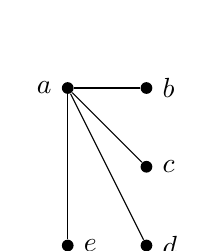
\begin{tikzpicture}
    \centering
    \node(B) at (1,0) [circle, fill, inner sep = 1.5pt, label=right:$b$] {};
    \node(C) at (1,-1) [circle, fill, inner sep = 1.5pt, label=right:$c$] {};
    \node(D) at (1,-2) [circle, fill, inner sep = 1.5pt, label=right:$d$] {};
    \node(E) at (0,-2) [circle, fill, inner sep = 1.5pt, label=right:$e$] {};
    \node(A) at (0,0) [circle, fill, inner sep = 1.5pt, label=left:$a$] {}
      edge [-, ] (B)
      edge [-, ] (C)
      edge [-, ] (D)
      edge [-, ] (E)
      ;
  \end{tikzpicture}
    \caption{Graph no extra connection}
\end{subfigure}
\hfill
\begin{subfigure}[b]{0.4\textwidth}
    \centering
  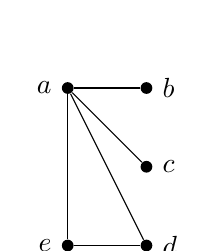
\begin{tikzpicture}
    \centering
    \node(B) at (1,0) [circle, fill, inner sep = 1.5pt, label=right:$b$] {};
    \node(C) at (1,-1) [circle, fill, inner sep = 1.5pt, label=right:$c$] {};
    \node(D) at (1,-2) [circle, fill, inner sep = 1.5pt, label=right:$d$] {};
    \node(E) at (0,-2) [circle, fill, inner sep = 1.5pt, label=left:$e$] {}
    edge [-, ] (D)
      ;
    \node(A) at (0,0) [circle, fill, inner sep = 1.5pt, label=left:$a$] {}
      edge [-, ] (B)
      edge [-, ] (C)
      edge [-, ] (D)
      edge [-, ] (E)
      ;
  \end{tikzpicture}
    \caption{Graph with extra connection}
\end{subfigure}
  \caption{Subgraph of $G^c$}
  \label{Q1}
\end{figure}


\begin{figure}
  \centering
  
  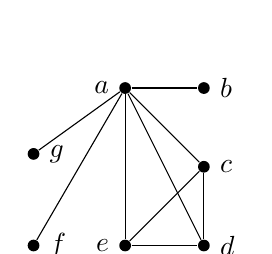
\begin{tikzpicture}
    \centering
    \node(B) at (1,0) [circle, fill, inner sep = 1.5pt, label=right:$b$] {};
    \node(C) at (1,-1) [circle, fill, inner sep = 1.5pt, label=right:$c$] {};
    \node(D) at (1,-2) [circle, fill, inner sep = 1.5pt, label=right:$d$] {}
      edge [-, ] (C)
      ;
    \node(E) at (0,-2) [circle, fill, inner sep = 1.5pt, label=left:$e$] {}
    edge [-, ] (D)
    edge [-, ] (C)
      ;
    \node(F) [left=of E] [circle, fill, inner sep = 1.5pt, label=right:$f$] {};
    \node(G) [above=of F] [circle, fill, inner sep = 1.5pt, label=right:$g$] {};
    \node(A) at (0,0) [circle, fill, inner sep = 1.5pt, label=left:$a$] {}
      edge [-, ] (B)
      edge [-, ] (C)
      edge [-, ] (D)
      edge [-, ] (E)
      edge [-, ] (F)
      edge [-, ] (G)
      ;
  \end{tikzpicture}
  \caption{A subgraph of $G$ with a vertex degree 6}
  \label{Q1:Vertex6}
\end{figure}

Divide all graph of 9 vertices into two cases

\begin{enumerate}
\item Those graph with minimum vertex degree smaller than or equal to 4.
\item Those graph with minimum vertex degree greater than 4
\end{enumerate}

We shall prove that for both cases our statement holds.

\emph{Case 1}

Let The vertex with minimum degree be $a$. Vertex degree of $a$ is smaller than 4, thus $a$ in $G^c$ must have vertex degree greater than or equal to 4. 

Consider the $G^c$ resented in figure \ref{Q1}, in which $a$ is the promised vertex. There are two cases:

\begin{enumerate}[label=\alph*)]
  \item There are no extra  line connecting $b,c,d,e$, which means in its complement, $G$, each one of $b,c,d,e$ are connected to all others, forming a isomorphic subgraph to $K_4$.
  \item There are at least one  line connectting two of the $b,c,d,e$. These two vertices and $a$ forms a isomorphic subgraph to $K_3$
\end{enumerate}

Thus our statement holds for case 1.

\emph{Case 2}

Graphs with the minimum vertex degree greater than four must have at least one vertex with degree greater than or equal to 6. 
If there is no vertices with degree greater than 6, then all vertex must have degree 5, which means the total vertex degree is an odd number, 45, contradicting handshaking lemma.

Let $a$ be the vertex with at least degree $6$ in graph $G$. Figure \ref{Q1:Vertex6} shows $a$ with 6 other vertices connected to it.

We know in a graph with 6 vertices, either it has a subgraph isomorphic to $K_3$ or its complement has one. For the subgraph consisted with $b,c,d,e,g,f$, if its compliment has a $K_3$ subgraph, we are done. If not, it must have a $K_3$ subgraph, and the vertex $a$ with its $K_3$ subgraph forms a $K_4$ subgraph. (See figure \ref{Q1:Vertex6})

\end{proof}

\newpage

\begin{problem}{2}
Let $G$ be a connected graph with vertices $\{v_1,\ldots,v_n\}$ and adjacency matrix $A$.
In this problem we define an \emph{embedded triangle} to be a subgraph isomorphic to $K_3$, and an \emph{embedded quadrilateral} to be a subgraph isomorphic to $C_4$.

\begin{enumerate}[label=\alph*)]
    \item \textbf{[3pts]} Prove by induction on $k$ that the $ij$-th entry of the matrix power $A^k$ counts the number of walks from $v_i$ to $v_j$ of length $k$.
    \item \textbf{[1pt]} Conclude that the trace of $A^2$ equals twice the number of edges of $G$, and that the trace of $A^3$ equals six times the number of embedded triangles of $G$, under the further assumption that $G$ is simple.
    \item \textbf{[1pt]} Discuss: what precisely goes wrong when trying to generalize this technique to count embedded quadrilaterals?
\end{enumerate}

\end{problem}

\subsection*{a)}
\begin{proof}
    We shall prove by induction on $k$ that the $ij$-th entry of the matrix power $A^k$ counts the number of walks from $v_i$ to $v_j$ of length $k$.
    
    \emph{Base case:} $k=1$, $A^1$ is the adjacency matrix of $G$. The number of walks of length 1 connecting $v_i, v_j$ is the number of edges between them, which, by definition, is the $i,jth$ entry of $A$. 
    
    \emph{Inductive step:} Assume the statement holds for $k=p$, we shall prove it holds for $k=p+1$. 
    
    Let $A^p_{i,j}$ donote the $ij-th$ entry of $A^p$. 

    Consider a walk with length $p+1$ from $v_i$ to $v_j$. $A^p_{i, 1}$ denotes the number of path with length $p$ from $v_i$ to $v_1$, and $A_{1, j}$ denotes the number of path with length $n$ from $v_1$ to $v_j$.

    Thus the number of path with length $p+1$ from $v_i$ to $v_j$ that pass through $v_1$ at the secound last step is $A^p_{i,1} \cdot A_{i,j}$
     
    Similarly, $A^p_{i, m} \cdot A_{m,j}$, denotes the number of path with length $p+1$ from $v_i$ to $v_j$ that pass through $v_m$ at the secound last step. $\sum^{n}_{m=1} A^p_{i,m}\cdot A_{m,j} $, their sum thus is the number of all walks of length $p+1$ from $v_i$ to $v_j$.
    
\end{proof}

\subsection*{b)}

\subsubsection*{1}

The number of walks of length 2 connecting $v_i$ to itself is its order. Thus the trace of $A^2$ equals total vertices order of $G$.

One edge would contribute to two vertex order, thus the trace of $A^2$ equals twice the number of edges of $G$.

\subsubsection*{2}

Consider a triangle connecting vertices $v_1, v_2, v_3$. There are two walks from $v_1$ to itself due to this triangle: $v_1 \rightarrow v_2 \rightarrow v_3$ and $v_1 \rightarrow v_3 \rightarrow v_2$; likewise for $v_2$ and $v_3$. Thus a single trianlge contributes 6 closed path.

Trace of $A^3$ is the sum of all closed path of length 3. Thus the trace of $A^3$ equals six times the number of embedded triangles of $G$.


\subsection*{c)}

Counting total number of triangles with the trace of $A^3$ works only if the presense of triangle, and no other shapes or entities, would result in certain number walk of length 3 starting and ending with same vertex. However, many different shapes would result a closed path of length 4, such as traversing the same edge four times.

\end{document}

